\documentclass[11pt,letterpaper,boxed]{hmcpset}
\usepackage{fullpage}
\setlength{\parskip}{6pt}
\setlength{\parindent}{0pt}
\usepackage[margin=1in]{geometry}
\usepackage{graphicx}
\usepackage{enumerate}
\usepackage{marvosym}
\usepackage{amssymb}
\usepackage{wasysym}
\usepackage{gensymb}
\usepackage{mathrsfs}
\usepackage{scrextend}
\usepackage{mathtools}
\usepackage{pgfplots}
\usepackage{xspace}
\usepackage[colorlinks]{hyperref}

\makeatletter
\renewcommand*\env@matrix[1][*\c@MaxMatrixCols c]{%
   \hskip -\arraycolsep
   \let\@ifnextchar\new@ifnextchar
   \array{#1}}
\makeatother

% --- style --- %
\renewcommand{\labelenumi}{{ (\alph{enumi})}}
\newcommand{\sand}{\quad \mbox{ and } \quad}
%\newcommand{\ds}{\displaystyle}
\allowdisplaybreaks

% --- making \xi look less awful --- %
\DeclareSymbolFont{CMletters}{OML}{cmm}{m}{it}
\DeclareMathSymbol{\xi}{\mathord}{CMletters}{"18}

% --- math --- %
\newcommand{\Z}{\mathbb{Z}}
\newcommand{\R}{\mathbb{R}}
\newcommand{\C}{\mathbb{C}}
\newcommand{\Q}{\mathbb{Q}}


\newcommand{\Lt}[1]{\mathcal{L}\crb{#1}}
\newcommand{\ilt}[1]{\mathcal{L}^{-1}\crb{#1}}

\newcommand{\pn}[1]{\left( #1 \right)}
\newcommand{\sqb}[1]{\left[ #1 \right]}
\newcommand{\crb}[1]{\left\{ #1 \right\}}
\newcommand{\lra}[1]{\left\langle #1 \right\rangle}
\newcommand{\magn}[1]{\left\lVert #1 \right\rVert}

\newcommand{\pdr}[2]{\frac{\partial #1}{\partial #2}}
\newcommand{\im}[1]{\text{im}\pn{#1}}
\newcommand{\m}[1]{\Z/#1\Z}

\newcommand{\VEC}[1]{\ensuremath{\mathbf{#1}}\xspace}
\DeclareMathOperator{\proj}{proj}
\newcommand{\vectorproj}[2][]{\proj_{\VEC{#1}}\VEC{#2}}

\newenvironment{amatrix}[1]{%
  \left(\begin{array}{@{}*{#1}{c}|c@{}}
}{%
  \end{array}\right)
}

\makeatletter
\renewcommand*\env@matrix[1][*\c@MaxMatrixCols c]{%
  \hskip -\arraycolsep
  \let\@ifnextchar\new@ifnextchar
  \array{#1}}
\makeatother

\newcommand{\spn}[1]{\text{span}\pn{#1}}

\newcommand*\Heq{\ensuremath{\overset{\kern2pt H}{=}}}

\name{Box \#$\rule{1cm}{0.15mm}$}
\class{Math 65 Section 1}
\assignment{Homework 8}
\duedate{29 May 2018}

\begin{document}

%\begin{center}
\noindent\textbf{Collaborators:} 
%\end{center} 

\begin{problem}[1.]  Write down a system of linear, homogeneous, first-order,
  constant-coefficient differential equations that could support the
  following graph.  The straight trajectories (and their orientations)
  are the only ones that you must preserve.  The large arrows are just
  meant to show the general trend of the trajectories in the rest of
  the phase plane.  Also, use pplane or some other
  computer program to draw some solution trajectories for your
  differential equations to show that they match the diagram.


\centering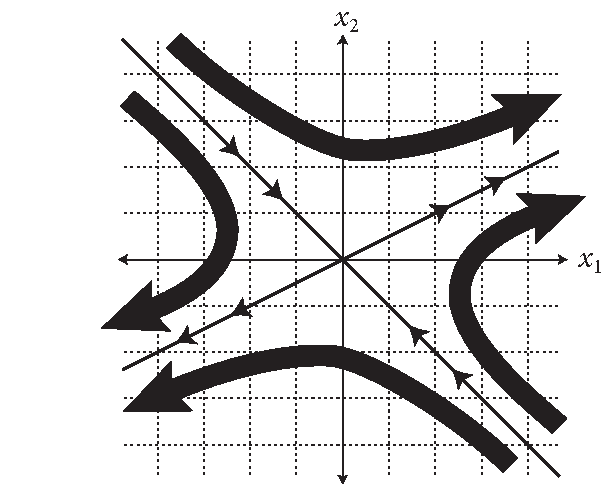
\includegraphics[width=4in,keepaspectratio=true]{./hw8phaseplane}

\end{problem}
%

\begin{solution}
\vfill
\end{solution}
\newpage

\begin{problem}[2.] 
\parbox{0.575\textwidth}{ An automobile suspension system can be modeled by a coupled mass-spring system as shown in the diagram, where $m_1$ is the car body, $m_2$ the wheel/tire assembly, and the dashpot $c$ is a shock absorber:
 \begin{eqnarray}
 m_1 \, x''  & = &  -k_1 (x-y)  - c(\dot{x} - \dot{y}) \\
 m_2 \, y'' &  = &  - k_2 y  - k_1 (y-x) - c(\dot{y} - \dot{x})
 \end{eqnarray}
 where $x$ and $y$ denote displacement from static equilibrium for mass $m_1$ and $m_2$, respectively (arrows indicate the positive direction), 
$k_1$ and $k_2$ are spring constants, and $c > 0$ is the damping coefficient.
      }
   \parbox{0.45\textwidth}{
 \[  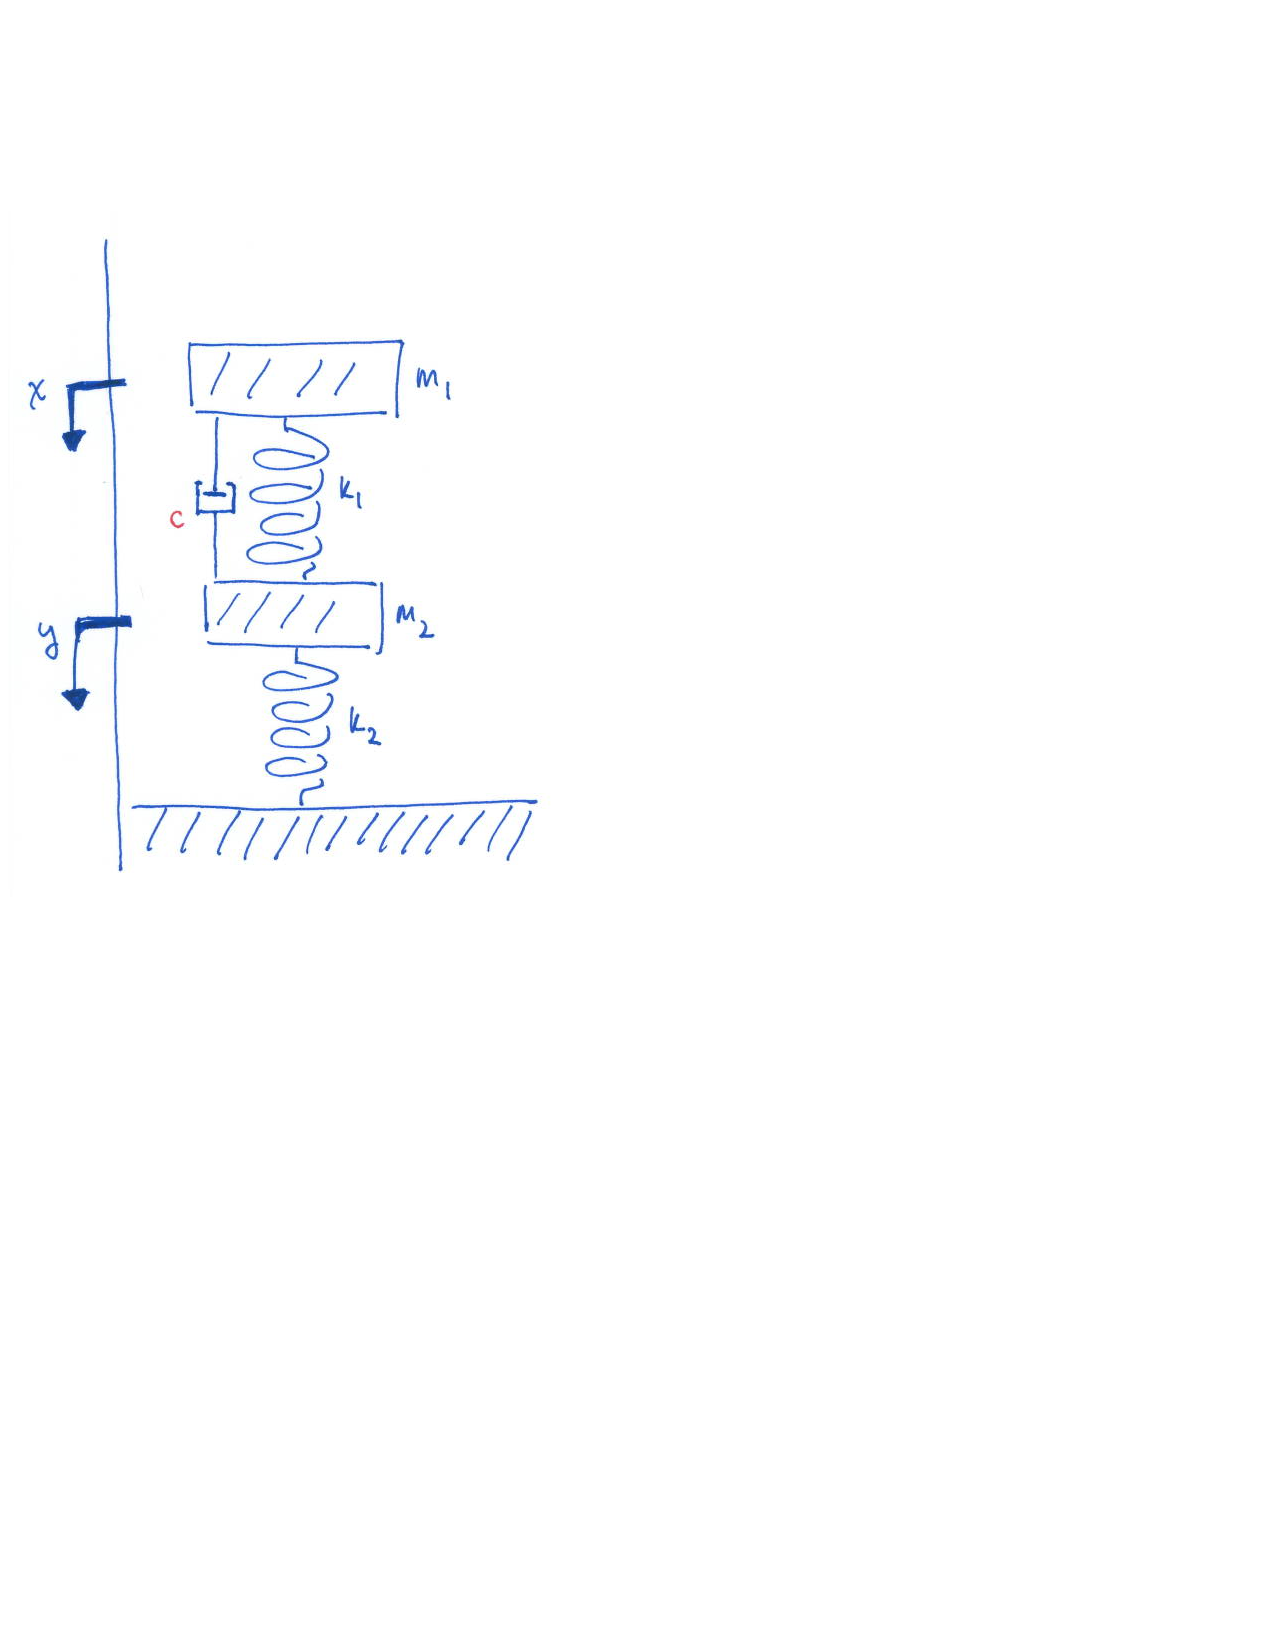
\includegraphics[width=0.35\textwidth]{./suspensionmodel2}  \]
 }

\begin{enumerate}
\item[(a)]   Rewrite the system of second order DEs (1)-(2) as a first-order system $\mathbf{x} ' = A \, \mathbf{x}$ and identify the matrix $A$. 
Note: Each second order DE should correspond to  two first-order equations so we are expecting a $4 \times 4$ matrix $A$.
\item[(b)] Assume $c = 0$ (no damping) and use a calculator or computer to determine the eigenvalues of your matrix $A$ when $m_1=m_2=1, k_1=3, k_2=2$. Do these eigenvalues seem appropriate? 

\item[(c)] Suppose we add damping, say $c=4$. What are the eigenvalues of $A$? What is different about the eigenvalues in this damped case vs.~the undamped case in  part (b)? 
\end{enumerate}
\end{problem}

\begin{solution}
\vfill
\end{solution}
\newpage

\begin{problem}[3.] The five points of this problem are dedicated to the clarity, precision, and style of your write up to the next problem.  This means first
working out all the details before writing up your solution (bonus points for particularly beautiful write ups!). 
\end{problem}

\begin{solution}
\vfill
\end{solution}
\newpage

\begin{problem}[4.] Solve the initial value problem
\[  \mathbf{x} \, ' = \begin{bmatrix} 0 & 2 \\ -2 & 0 \end{bmatrix} \, \mathbf{x} + \begin{bmatrix} \cos \omega t \\ \sin \omega t \end{bmatrix}  \]
where $\omega \neq 0$ and $\mathbf{x}_0 = \begin{bmatrix} a \\ b \end{bmatrix}$.
  Make sure your solution is valid for \textit{all} values of $\omega \neq 0$ (i.e., 
 be careful not to divide by $0$; if a given step leads to division by $0$ then you have to go back one step and reconsider the calculation more specifically in that case).  
\end{problem}

\begin{solution}
\vfill
\end{solution}
\newpage

\begin{problem}[5.]
Consider the following model for caffeine dynamics in the GI tract (stomach and intestines; $x$) and the bloodstream ($y$):
\begin{eqnarray*}
\dot{x} & = &   -kx +I(t),  \\
  \dot{y} & =  & kx-ky, 
  \end{eqnarray*}
where we have chosen the two rate constants to be equal ($k_1=k_2=k$) and $k>0$ and $I(t)$ is a forcing term.
Here $I(t)$ is the caffeine input rate and $x(0)=x_0, y(0)=y_0,$ are the initial concentration of caffeine in the GI tract ($x_0$) and bloodstream ($y_0$). 

\begin{enumerate}

\item[(a)] Write the system in matrix form $\mathbf{x}\, ' = A \, \mathbf{x} + \mathbf{F}$ and identify the matrix $A$ and forcing vector $\mathbf{F}$.  

\item[(b)] Solve the system  with $I(t)=0$ (for all $t$) as a ``cascade" by first solving for $x$, then substituting that solution into the $\dot{y}$ equation and solving for $y$.


\item[(c)] Use your work from Part (b) to find a fundamental matrix $\Psi(t)$ and then $e^{At}$.  Note: You have done most of the work already in part (b).


\item[(d)] Use Variation of Parameters 
to solve for $x$ and $y$ when $I(t)=1$ (steady drip) and $x_0=y_0=0$ (initially no caffeine). Graph your
solutions when $k=2$ (using a calculator/computer is fine).   What happens at $t \to \infty$?
\end{enumerate}

 \end{problem}

\begin{solution}
\vfill
\end{solution}
\newpage

\begin{problem}[6.]
\bigskip
\hrule
\bigskip

\noindent \textbf{Definition} An \textit{equilibrium point} for the system 
\[ \mathbf{x}' = \mathbf{f}(\mathbf{x}) \] 
is a state $\mathbf{x}_0$ such that $\mathbf{f}(\mathbf{x}_0)=\mathbf{0}$. The term comes from the fact that $\mathbf{f}(\mathbf{x}_0)=\mathbf{0}$ implies 
$\mathbf{x}' = \mathbf{0}$, hence the states of the system will not change and therefore the system is in an equilibrium state.

\bigskip
\hrule
\bigskip


Write each of the following differential equations as an equivalent  first-order system. Find all equilibrium points (if any) for each system.
\begin{enumerate}
\item[(a)] (\textbf{van der Pol})
$$\ddot{u} + \lambda  (u^2 - 1) \dot{u} + u = 0$$ 
where $\lambda > 0$. This is an important model in the theory of oscillations, famous enough to have its own wiki page (Balthasar van der Pol considered the equation in trying to model oscillatory electrical activity in the heart).
 \item[(b)] (\textbf{Pendulum}) 
\[  \theta'' + c \theta' + \lambda \sin \theta = 0 \]
which models a damped pendulum where $\theta(t)$ is the angle from static equilibrium, $c > 0$ is a damping constant, and $\lambda = \sqrt{g/L}$.   
\end{enumerate}
Note: These are nonlinear DEs so they will not be linear systems, but you can still use the same method as we used for the mass-spring equation to ``systemify".
\end{problem}

\begin{solution}
\vfill
\end{solution}
\newpage

\begin{problem}[7.] In Math 45 you were introduced to the SIR (Susceptible- Infected-Recovered) Model:
\begin{eqnarray*}
\dot{S} & = & -\alpha I S \\
\dot{I} & = &  \alpha I S - \beta I  \\
\dot{R} & = & \beta I
\end{eqnarray*}
where $\alpha,\beta  > 0$ are constants (infection and recovery rate, respectively).   
This is a model for a disease that propagates through a community (e.g., flu on a college campus during a particular semester). Typically we scale by the total population so that
 \begin{enumerate}
\item[(a)] Show that for solutions of the model the total population $S+I+R$ remains constant. Hint: Let $N=S+I+R$. What is $\dot{N}$?
\item[(b)] Given the total population remains constant we typically scale by $N$ so that $0 \leq S,I,R \leq 1$ (i.e., they represent the fraction of the population that is any given state (susceptible to the disease, infected, or recovered). Assuming this is the case, find all equilibrium points of the system and explain what the
equilibrium points physically corresponds to with the population.
\end{enumerate} 
\end{problem}

\begin{solution}
\vfill
\end{solution}
\newpage

\end{document}
